\documentclass{article}
\usepackage{graphicx} % Required for inserting images
\usepackage{authblk} % For author affiliations
\usepackage{hyperref} % For hyperlinks
\usepackage[margin=1in]{geometry} % Standard margins

\title{Integrating Multiple Data Sources in Infectious Disease Modelling: Best Practices and Implementation}

\author[1]{Sam Abbott}
\author[2]{Punya Alahakoon}
\author[3]{Xiahui Li}
\author[4]{Dhorasso Junior Temfack Nguefack}
\author[5]{Michael Plank}
\author[6]{@working-group-members}
\author[7]{@workshop-participants}
\author[8]{Anne Presanis\thanks{Joint last authors}}
\author[9]{Anne Cori\footnotemark[1]}

\affil[1]{London School of Hygiene \& Tropical Medicine}
\affil[2]{University of Oxford}
\affil[3]{University of St Andrews}
\affil[4]{Trinity College Dublin}
\affil[5]{@working-group-affiliations}
\affil[6]{@workshop-participant-affiliations}
\affil[7]{University of Canterbury, New Zealand}
\affil[8]{MRC Biostatistics Unit, University of Cambridge}
\affil[9]{Imperial College London}

\date{\today}

\begin{document}

\maketitle

\begin{abstract}
Infectious disease modelling increasingly relies on integrating multiple data sources to improve parameter estimation and reduce uncertainty.
However, practitioners face complex choices about how to combine diverse data streams, from full joint modelling to modular approaches that fit sub-models separately before integration.
This paper provides a comprehensive framework for integrating multiple data sources in infectious disease modelling, with transmission intensity estimation as a key exemplar.
We review data source characteristics, present a structured workflow for model development, and compare integration approaches including joint modelling, evidence synthesis methods, and ensemble techniques.
Through worked case studies progressing from single data sources to multi-stream integration, we demonstrate how different data types provide complementary information for estimating parameters such as time-varying reproduction numbers and overdispersion.
We discuss computational considerations, model validation strategies, and practical implementation challenges.
Our modular framework emphasises parsimony, interpretability, and systematic assessment of conflict between data sources.
This work addresses a critical gap in the literature by providing practical guidance for infectious disease modellers on data integration choices, supported by reproducible examples and decision-making frameworks.
\end{abstract}

\section{Introduction}
% Lead: Sam Abbott

% Paragraph 1: Motivation and Context
% TODO: Value of multiple data sources in epidemic modelling
% TODO: Recent examples from COVID-19, mpox, Ebola
% TODO: Challenges of single data source limitations

% Paragraph 2: Current Approaches
% TODO: Pipeline vs joint modelling approaches
% TODO: Trade-offs between computational complexity and information gain
% TODO: Existing frameworks and their limitations

% Paragraph 3: Paper Scope and Contribution
This paper provides a comprehensive framework for integrating multiple data sources in infectious disease modelling, with practical implementation as the primary focus.
We use transmission intensity estimation—specifically time-varying reproduction numbers and overdispersion parameters—as a case study to demonstrate broader principles applicable across infectious disease modelling contexts.
Our approach encourages iterative model building, allowing practitioners to systematically assess the value of additional data sources while maintaining interpretability and computational tractability.
The framework addresses critical gaps in existing literature by providing domain-specific guidance and signposting to more generic resources for integration choices, validation strategies, and conflict resolution between data sources.

% Paragraph 4: Paper Structure
We first review data source characteristics and present a structured iterative workflow for model development that progresses from research question definition through process and observation DAG development to integration method selection.
We then compare integration approaches from full joint modelling to modular ensemble methods.
Three worked case studies demonstrate progressive complexity: single-source baselines, two-source integration, and multi-stream applications incorporating individual-level data.
Each case study follows our iterative workflow, demonstrating how DAG-based model development guides data integration decisions.

\section{Data Sources and Characteristics}
% Lead: Punya Alahakoon

We conducted a survey of workshop participants to systematically evaluate different data sources for infectious disease modelling.
This tool helps practitioners rate different data sources on quality, timeliness, and usefulness for modelling SARS-CoV-2.
By pooling expert opinions, we have created visual comparisons showing trade-offs between different data types, making it easier to decide which data to use when estimating transmissibility and identifying when different sources might conflict.

Participants evaluated candidate datasets across six main categories: basic metadata, scope, resolution, data quality, data utility, and practical considerations.
For each subcategory, experts assigned values between 0 and 5, selected appropriate categories, or provided free text responses.
We harmonised and ensembled these expert assessments to create overview tables and data analysis.

% TODO: Present survey results and expert consensus
% TODO: Create comprehensive table of data characteristics  
% TODO: Discuss taxonomy of data sources in infectious disease surveillance
% TODO: Analyse information content and complementarity
% TODO: Address preprocessing and standardisation requirements

\section{Workflow}
% Lead: Sam Abbott

\subsection{Overview}

We recommend following a structured, iterative workflow for multi-data source modelling (Figure~\ref{fig:workflow}).

\begin{figure}[htbp]
    \centering
    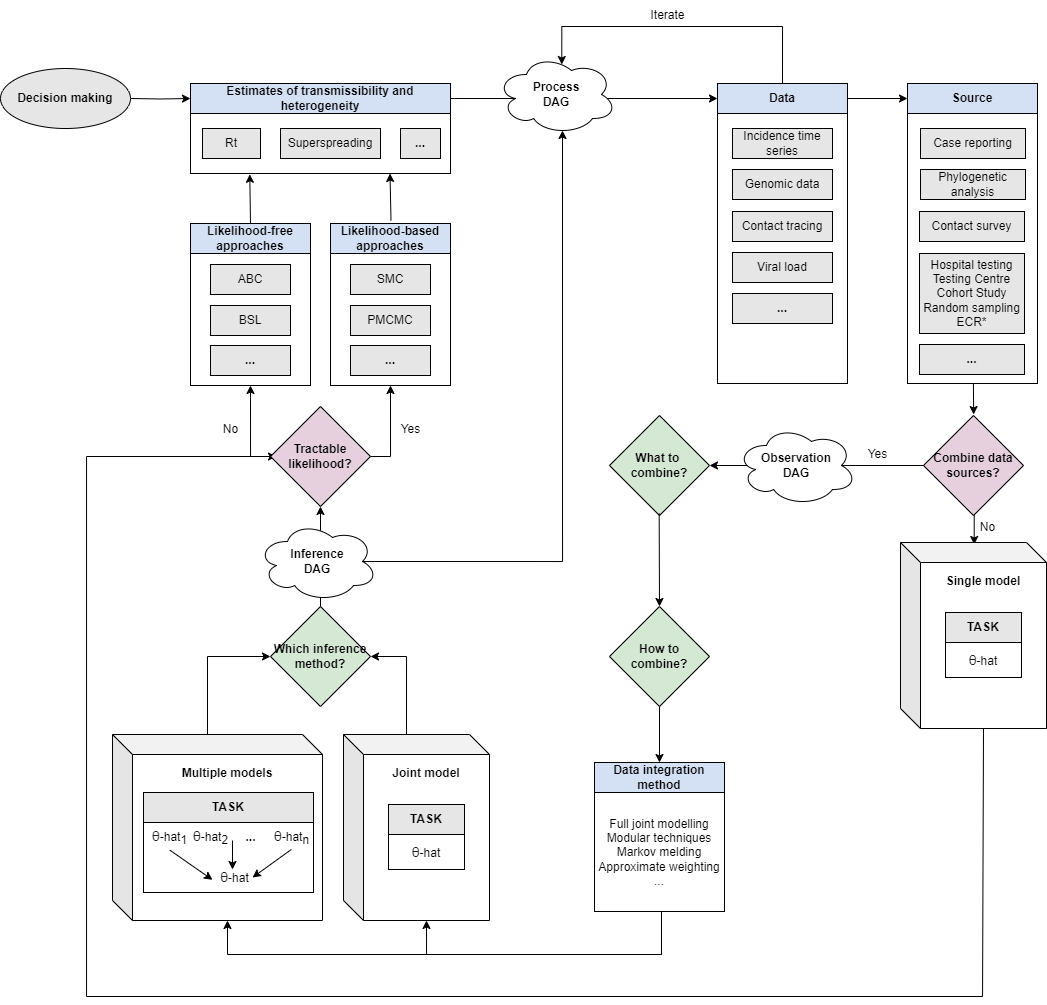
\includegraphics[width=\textwidth]{figures/workflow-schematic.png}
    \caption{Recommended workflow for integrating multiple data sources in infectious disease modelling. Begin by defining research questions and target estimands, proceed through iterative development of process and observation DAGs, and follow critical decisions about data integration and inference methods.}
    \label{fig:workflow}
\end{figure}
Start with a clear research question—such as estimating transmission intensity—and use systematic model development through directed acyclic graphs (DAGs) with iterative refinement.
We advocate this approach because it makes modelling choices transparent, assumptions explicit, and allows systematic assessment of additional data sources.

We recommend beginning with **decision making**: clearly define your research question and target estimands (e.g., time-varying reproduction number, overdispersion parameters).
Next, develop a **process DAG** representing the underlying epidemiological process, iterating on this representation as understanding develops.
Map available **data sources** to your process model, such as incidence time series, genomic data, contact tracing, viral load measurements, and serological surveys.
For each data source, develop an **observation DAG** linking the underlying process to observed data through measurement models and reporting mechanisms.
Different data sources may also impact your **process DAG** assumptions, such as if you can collapse your approach from individual-level to population-level.

Once you have developed your process and observation DAGs, proceed to **model specification and validation**, including prior specification, parameter identifiability assessment, and diagnostic approaches.
You then face the key decisions: **"What to combine?"** and **"How to combine?"**
If combining multiple sources is not beneficial or feasible, you can proceed to single-source modelling and combination of estimates.
If integration is warranted, select among data integration methods including full joint modelling, modular techniques, Markov melding, or approximate weighting approaches.
Finally, fit your model and evaluate its performance through posterior predictive validation and sensitivity analysis.

In the following sections, we will discuss each of these steps in more detail.

\subsection{Research Question and Target Estimands}
% TODO: Defining clear research objectives
% TODO: Specifying target parameters and estimands
% TODO: Connecting questions to policy needs
% TODO: Setting scope and boundaries

\subsection{Process DAG Development}
% TODO: Representing epidemiological processes
% TODO: Causal relationships and assumptions
% TODO: Iterative refinement based on understanding
% TODO: Incorporating biological mechanisms

\subsection{Data Source Mapping}
% TODO: Cataloguing available data streams
% TODO: Assessing data characteristics and biases
% TODO: Linking data to process components
% TODO: Evaluating complementarity and redundancy

\subsection{Observation DAG Construction}
% TODO: Measurement models and reporting processes
% TODO: Delays and missing data mechanisms
% TODO: Linking latent processes to observations
% TODO: Accounting for data collection protocols

\subsection{Model Specification and Validation}
% TODO: Bayesian workflow principles
% TODO: Prior specification and prior predictive checks
% TODO: Parameter identifiability assessment
% TODO: Model criticism and diagnostic approaches
% TODO: Posterior predictive validation
% TODO: Cross-validation strategies
% TODO: Sensitivity analysis frameworks

\subsection{Data Integration Choices}
% Lead: Anne Presanis

\begin{itemize}
    \item Different possible choices for integrating/ensembling inference from multiple data sources
    \begin{itemize}
        \item Full joint model fitted, regardless of whether you have already fitted separate sub-models
        \item Conditionally independent sub-models each fitted separately, then integrated
        \begin{itemize}
            \item Meta-analysis of separate estimates
            \item Weighted averaging / ensembling
            \item Markov melding
        \end{itemize}
    \end{itemize}
    \item Depends on whether you are starting from scratch, from an existing model for one data source to which you want to add others, or whether you have multiple alternative sets of existing inferences from different data sources that you want to combine
    \item General principle that modular model building (De Angelis et al, 2015; Birrell et al, 2018; Goudie et al, 2019; De Angelis \& Presanis, 2019; Nicholson et al, 2022, Liu \& Goudie, 2025) is preferable, since:
    \begin{itemize}
        \item Easier to understand lack of fit, model misspecification or convergence issues from simpler sub-models individually
        \item Occam's razor - principle of parsimony, start from simplest model and build complexity up only as far as needed
        \item Adding sub-models in one at a time allows for assessment of consistency/conflict between sub-models sequentially
        \item Computational efficiency - rather than fitting full joint models after fitting the sub-models, use the posterior samples from the sub-models to obtain your full joint model (melding or ?)
    \end{itemize}
    \item Choice of likelihood function (or other objective function) therefore depends on options above on where you are starting from (existing models/sub-models or from scratch)
    \item And model development is a cycle of model building and model criticism
\end{itemize}

% TODO: Add practical examples of each approach
% TODO: Include decision framework for choosing integration method

\subsection{Fitting Choices}
% Lead: Anne Presanis, with Dhorasso and Xiahui

% Paragraph 1: Define the Task
% TODO: Summarise common features of epidemiological models
% TODO: Time-varying processes, underreporting, measurement errors
% TODO: Heterogeneity in spatial dynamics and population structure
% Transition: These challenges drive development of statistical methodologies based around likelihood functions

% Paragraph 2: Tools for Tractable Likelihood Functions
% TODO: MCMC and its variants for joint models
% TODO: Particle MCMC (pMCMC) for state-space formulations
% TODO: Sequential Monte Carlo (SMC) approaches
% TODO: Variational inference (VI) and INLA for specific model classes

% Paragraph 3: Tools for Intractable Likelihood Functions
% TODO: Approximate Bayesian Computation (ABC-MCMC, ABC-SMC)
% TODO: ABC with history matching
% TODO: Bayesian Synthetic Likelihood (BSL)
% TODO: Simulation-based inference approaches

% Paragraph 4: Selecting the Right Tool
% TODO: Trade-offs between computational complexity, accuracy, bias
% TODO: Interpretability and implementation ease considerations
% TODO: Decision-making frameworks for method selection

% Paragraph 5: Practical Implementation
% TODO: Software implementations and availability
% TODO: Diagnostic tools and convergence assessment
% TODO: Computational resource requirements
% TODO: Reference to inference subpanel workflow figure

\section{Practical Considerations}
% Lead: Sam Abbott

\subsection{Communication and Interpretation}
% TODO: Visualisation strategies for multi-source results
% TODO: Conveying uncertainty and methodological choices
% TODO: Transparent communication of limitations and assumptions
% TODO: Audience-specific communication approaches
% TODO: Highlighting individual data source contributions
% TODO: Standardised reporting templates and best practices
% TODO: Communicating integration method choices and rationale

\section{Case Studies}
% Lead: Anne Cori
% Case Study 0: Base Model - Cases Only
\subsection{Overview}

\subsection{Case Study 0: Base Model - Cases Only}
% TODO: Establish baseline single-source model
% TODO: Parameter estimation and uncertainty quantification
% TODO: Comparison framework for multi-source improvements


% Case Study 1: Two Data Sources
\subsection{Case Study 1: Cases and Deaths}
% TODO: Basic joint model formulation
% TODO: Parameter identifiability improvements
% TODO: Complete implementation with real data

% Case Study 2: Three Data Sources
\subsection{Case Study 2: Cases, Deaths, and Wastewater}
% TODO: Handling different observation processes
% TODO: Conflict resolution strategies
% TODO: Add sensitivity analyses

% Case Study 3: Incorporating Individual-Level Data
\subsection{Case Study 3: Cases and Transmission Pairs}
% TODO: Estimating overdispersion parameters
% TODO: Computational challenges and solutions
% TODO: Link to existing software tools

\section{Practical Considerations}
% Lead: Sam Abbott

% TODO: Real-time implementation challenges
% TODO: Data quality and missingness
% TODO: Model validation strategies
% TODO: Communication of integrated results
% TODO: Add checklist for practitioners

\section{Discussion}

\subsection{Summary of Our Approach}
% TODO: Recap key elements of the framework
% TODO: Highlight novel contributions (workflow, survey, case studies)
% TODO: Emphasise practical focus and modular philosophy
% TODO: Summarise main recommendations and best practices

\subsection{Comparison with Existing Literature}
% TODO: Position relative to pipeline vs joint modelling literature
% TODO: Relationship to evidence synthesis and meta-analysis methods
% TODO: Comparison with ensemble forecasting approaches
% TODO: Distinguish from existing reviews and methodological papers
% TODO: Compare with other multi-source integration frameworks

\subsection{Strengths and Limitations}
% TODO: Strengths: Modular framework, practical focus, worked examples
% TODO: Strengths: Integration of diverse methodological approaches
% TODO: Strengths: Expert survey and empirical evidence base
% TODO: Limitations: Model selection and validation challenges
% TODO: Limitations: Dependence on data quality and availability
% TODO: Limitations: Computational considerations and scalability

\subsection{Outstanding Challenges and Future Directions}
% TODO: Real-time implementation constraints and solutions
% TODO: Computational scalability for large-scale integration
% TODO: Methodological gaps in current approaches
% TODO: Emerging data sources and integration needs
% TODO: Community standards and best practices
% TODO: Research priorities and next steps

\section{Conclusions}
% TODO: Summary of key contributions and recommendations
% TODO: Practical impact for infectious disease modelling community
% TODO: How this framework advances the field
% TODO: Main takeaways for practitioners
% TODO: Call to action for standardisation and best practices

\section{Acknowledgements}
@placeholder

\section{References}
@placeholder

\end{document}
